\documentstyle[11pt,epsfig,fancybox,semcolor,semlayer,doublespace,portrait]
{seminar}
\input clp_utils

\def\ys{$\Upsilon(1S)$}
\def\yss{$\Upsilon(2S)$}
\def\ysss{$\Upsilon(3S)$}
\def\gamee{$\Gamma_{e^+e^-}$}

% The following strings are needed by the title page and 
% page style definitions in map_utils.tex
\newcommand{\talktitle}[0]{Event Accounting for $\Gamma_{ee}$ and R Measurements}
\newcommand{\fmttitle}[0]{}
\newcommand{\conftitle}[0]{November 1 CLEO PTA}
\newcommand{\myname}[0]{Jim Pivarski}
\newcommand{\affila}[0]{Cornell University}
\newcommand{\talkdate}[0]{November 1, 2002}

\pagestyle{conference}   % From clp_utils.tex

% slide magnification
\slidesmag 1

%%%%%%%%%%%%%%%%%%%%%%%%%%%%%%%%%%%%%%%%%%%%%%%%%%%%%%%%%%%%%%%%%%%%%%%%%%%
% Start document
\begin{document}

% Set page size
\slideheight 7.0in
\slidewidth 8.8in 

% Set array stretch
\renewcommand{\arraystretch}{0.3}
\renewcommand{\slidetopmargin}{0.4in}
\renewcommand{\slidebottommargin}{0.9in}


%%%%%%%%%%%%%%%%%%%%%%%%%%%%%%%%%%%%%%%%%%%%%%%%%%%%%%%%%%%%%%%%%%%%%%%%%%%

\begin{slide*}

\slideframe{}
\slideframe*[\dkblue]{Oval}

\begin{center}
\vspace{4 cm}
{\Huge \black Event Accounting \\ for $\Gamma_{ee}$ and R Measurements } \\
\vspace{1 cm}
{\LARGE \black	Jim Pivarski } \\
% \vspace{0.25 cm}
% {\LARGE	Ritchie Patterson } \\
% \vspace{0.25 cm}
% {\LARGE	Karl Berkelman } \\
\vspace{2 cm}
\conftitle \\
{\large \black \talkdate}

\end{center}

\end{slide*}

% %%%%%%%%%%%%%%%%%%%%%%%%%%%%%%%%%%%%%%%%%%%%%%%%%%%%%%%%%%%%%%%%%%%%%%%%%%%

% \begin{slide*}

% \slideframe{}
% \slideframe*[\dkblue]{Oval}
% \huge
% \heading{Outline}
% \vspace{1 cm}

% \begin{center}
% \begin{minipage}[t]{12 cm}
% \begin{itemize}
% \LARGE \item {\huge Motivation: verify lattice QCD!}
% \LARGE \item {\huge 2 out of 3 Resonances Scanned}
% \LARGE \item {\huge Energy Calibration Systematics}
% \LARGE \item {\huge Other Systematics / Work to be Done}
% \end{itemize}
% \end{minipage}
% \end{center}

% \end{slide*}
 
%%%%%%%%%%%%%%%%%%%%%%%%%%%%%%%%%%%%%%%%%%%%%%%%%%%%%%%%%%%%%%%%%%%%%%%%%%%

\begin{slide*}

\slideframe{}
\slideframe*[\dkblue]{Oval}
\huge
\heading{Goal and Conclusions}

\begin{minipage}[t]{\linewidth}
\Huge

\vspace{1 cm}

Goal: to understand what events make up the off-resonance data set.

\vspace{1 cm}

\begin{center}
  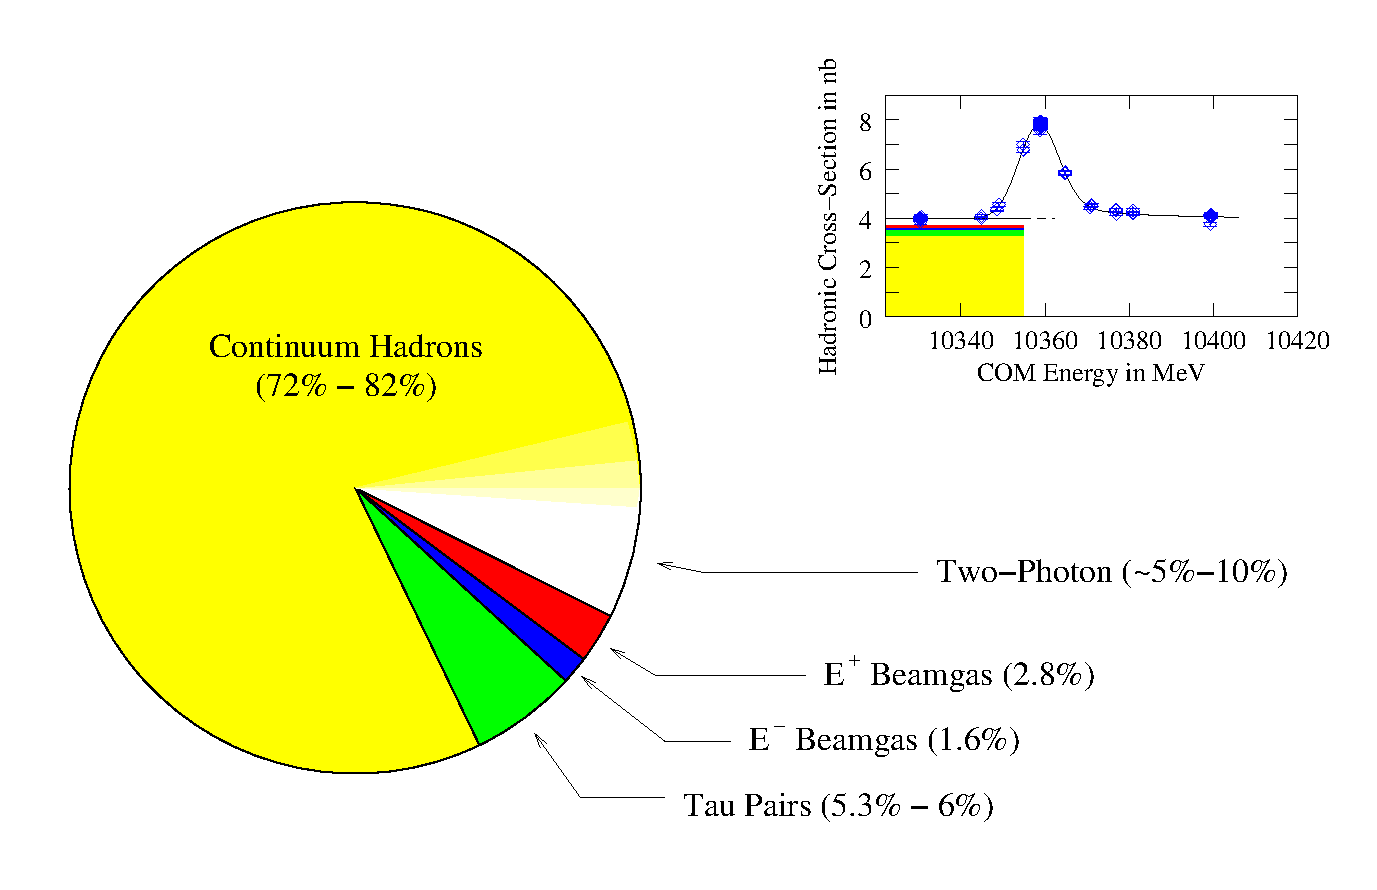
\includegraphics[width=\linewidth]{pie.eps}
\end{center}

\end{minipage}

\end{slide*}

%%%%%%%%%%%%%%%%%%%%%%%%%%%%%%%%%%%%%%%%%%%%%%%%%%%%%%%%%%%%%%%%%%%%%%%%%%%

\begin{slide*}

\slideframe{}
\slideframe*[\dkblue]{Oval}
\huge
\heading{What do I have to work with?}

\begin{minipage}[t]{\linewidth}
\LARGE

\vspace{1 cm}

\begin{flushleft}
\begin{itemize}
  \item Highly efficient cuts on beamwall/gas/cosmic rays \\
	($>$ 99\% of hadron MC pass, $\sim$1.3\% of beamwall/gas/cosmics
	pass, AFTER hadron subcollection cuts)

\vspace{0.5 cm}

  \item 17 pb$^{-1}$ sample of off-resonance data ($\Upsilon(3S)$ Dec 25 scan)

  \item Lots of continuum and tau Monte Carlo

  \item 3 hours of electron single-beam data \\
	40 minutes of positron single-beam data

\end{itemize}
\end{flushleft}

\end{minipage}

\end{slide*}

%%%%%%%%%%%%%%%%%%%%%%%%%%%%%%%%%%%%%%%%%%%%%%%%%%%%%%%%%%%%%%%%%%%%%%%%%%%

\begin{slide*}

\slideframe{}
\slideframe*[\dkblue]{Oval}
\huge
\heading{Highly-Efficient Cuts}

\begin{minipage}[t]{\linewidth}
\LARGE

\begin{tabular}{l c r}
  \begin{minipage}{3.5 in}
    \huge
    First two use the set of all track intersections in rphi.
  \end{minipage}
  & \hspace{0.5 in} & 
  \begin{minipage}{1 in}
    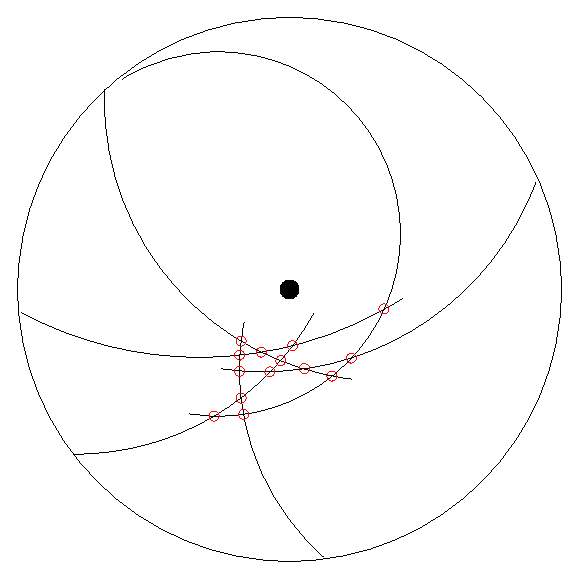
\includegraphics[width=\linewidth]{crossings_2d.eps}
  \end{minipage}
\end{tabular}

\vspace{0.5 cm}

\begin{flushleft}
\begin{itemize}
  \item \begin{tabular}{l c r}
  \begin{minipage}{3 in}
    \begin{flushleft}
    \Large
    {\bf Closest intersection \\ \hspace{1 cm} to beamspot $<$ 5 mm} \\
    Cuts out most cosmics and ALL beamwall
    \end{flushleft}
  \end{minipage}
  & \hspace{0.5 in} & 
  \begin{minipage}{1.5 in}
    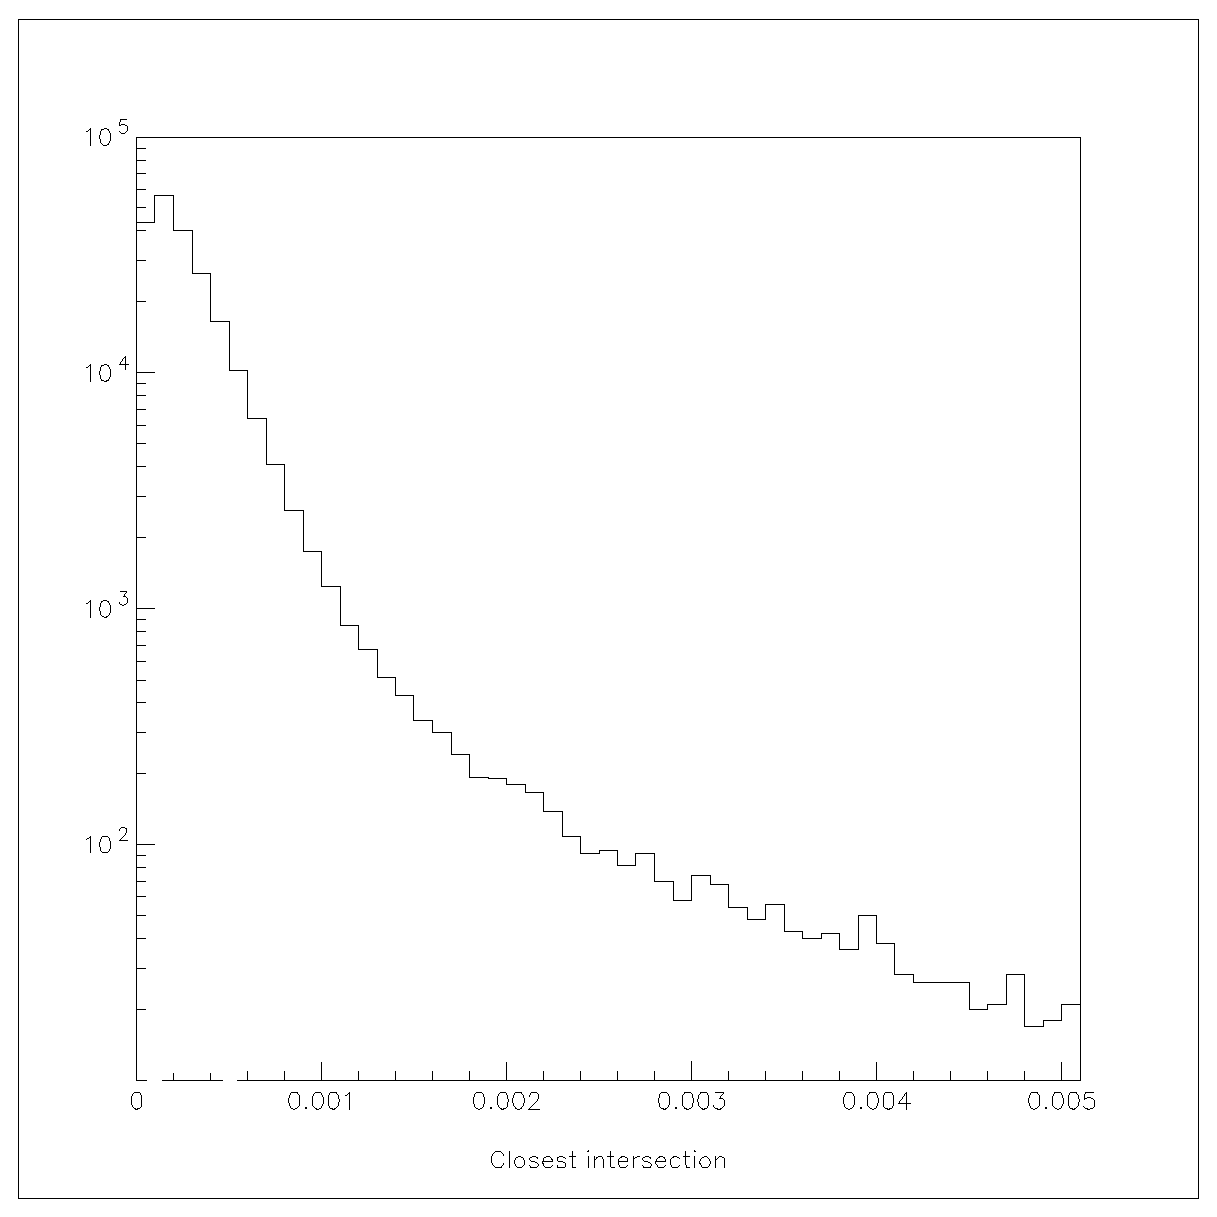
\includegraphics[width=\linewidth]{closest_intersection2.eps}
  \end{minipage}
\end{tabular}

  \item \begin{tabular}{l c r}
  \begin{minipage}{3 in}
    \begin{flushleft}
    \Large
    {\bf $\big|$ Weighted average Z \\ \hspace{1 cm} of intersections $\big|$ $<$ 5 cm} \\
    The weight includes z-mismatch and distance
    of intersection from beamspot.
    \end{flushleft}
  \end{minipage}
  & \hspace{0.5 in} & 
  \begin{minipage}{1.5 in}
    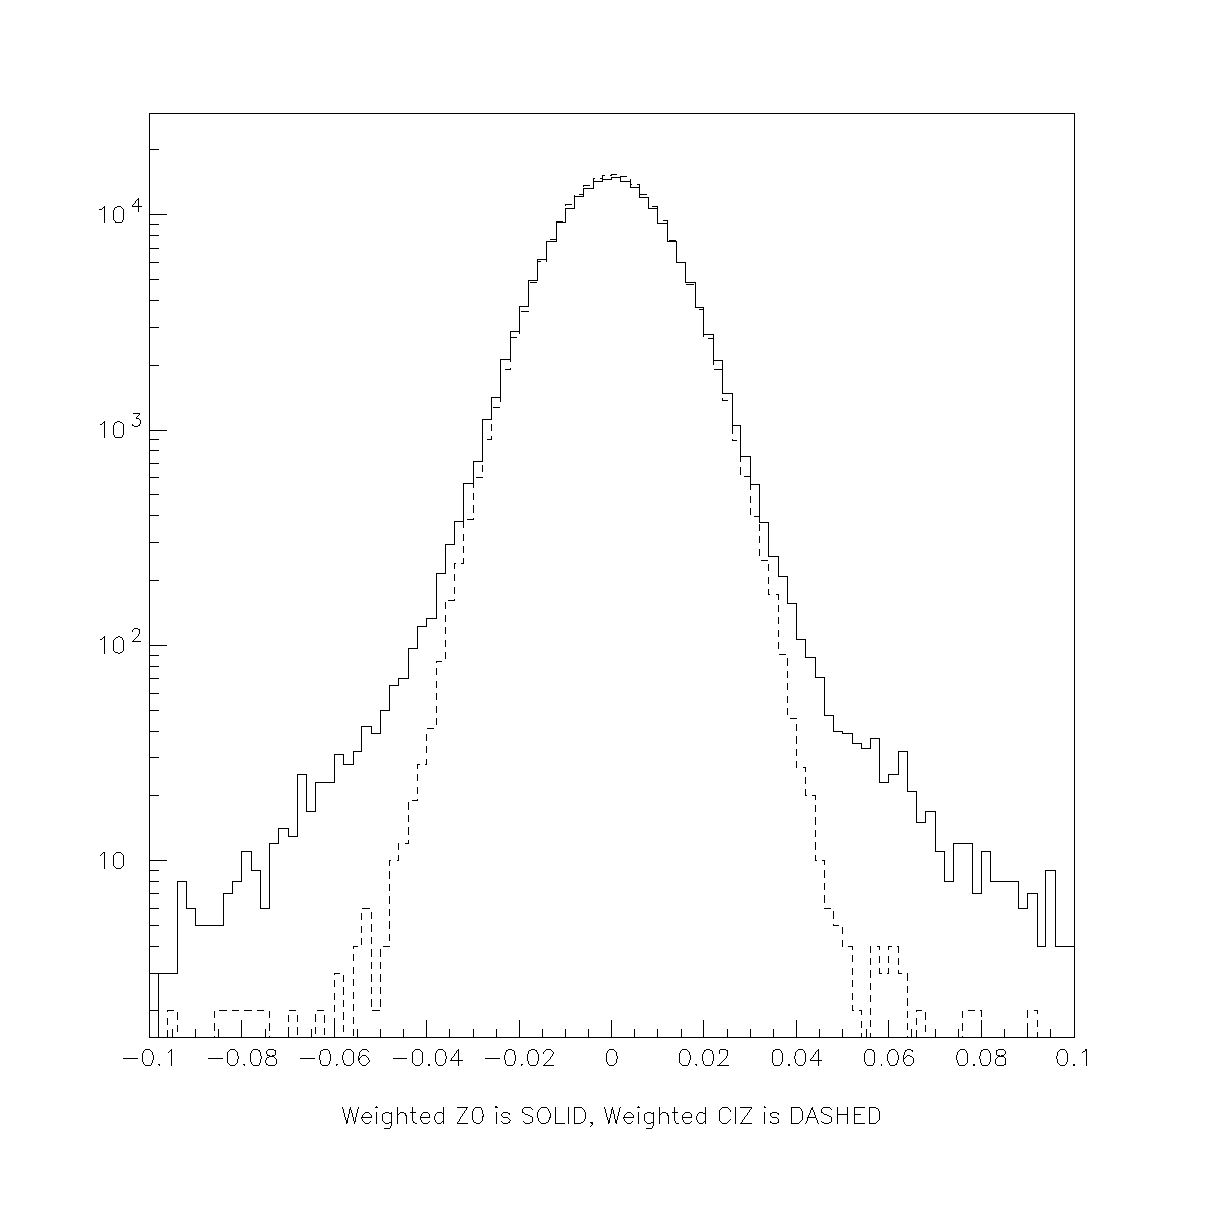
\includegraphics[width=\linewidth]{weighted_z2.eps}
  \end{minipage}
\end{tabular}

  \item \begin{tabular}{l c r}
  \begin{minipage}{3 in}
    \begin{flushleft}
    \Large
      {\bf Neutral energy exactly zero} \\
      90\% of beamgas has exactly zero neutral energy, $<$ 1\% of Monte Carlo does
    \end{flushleft}
  \end{minipage}
  & \hspace{0.5 in} & 
  \begin{minipage}{1.5 in}
    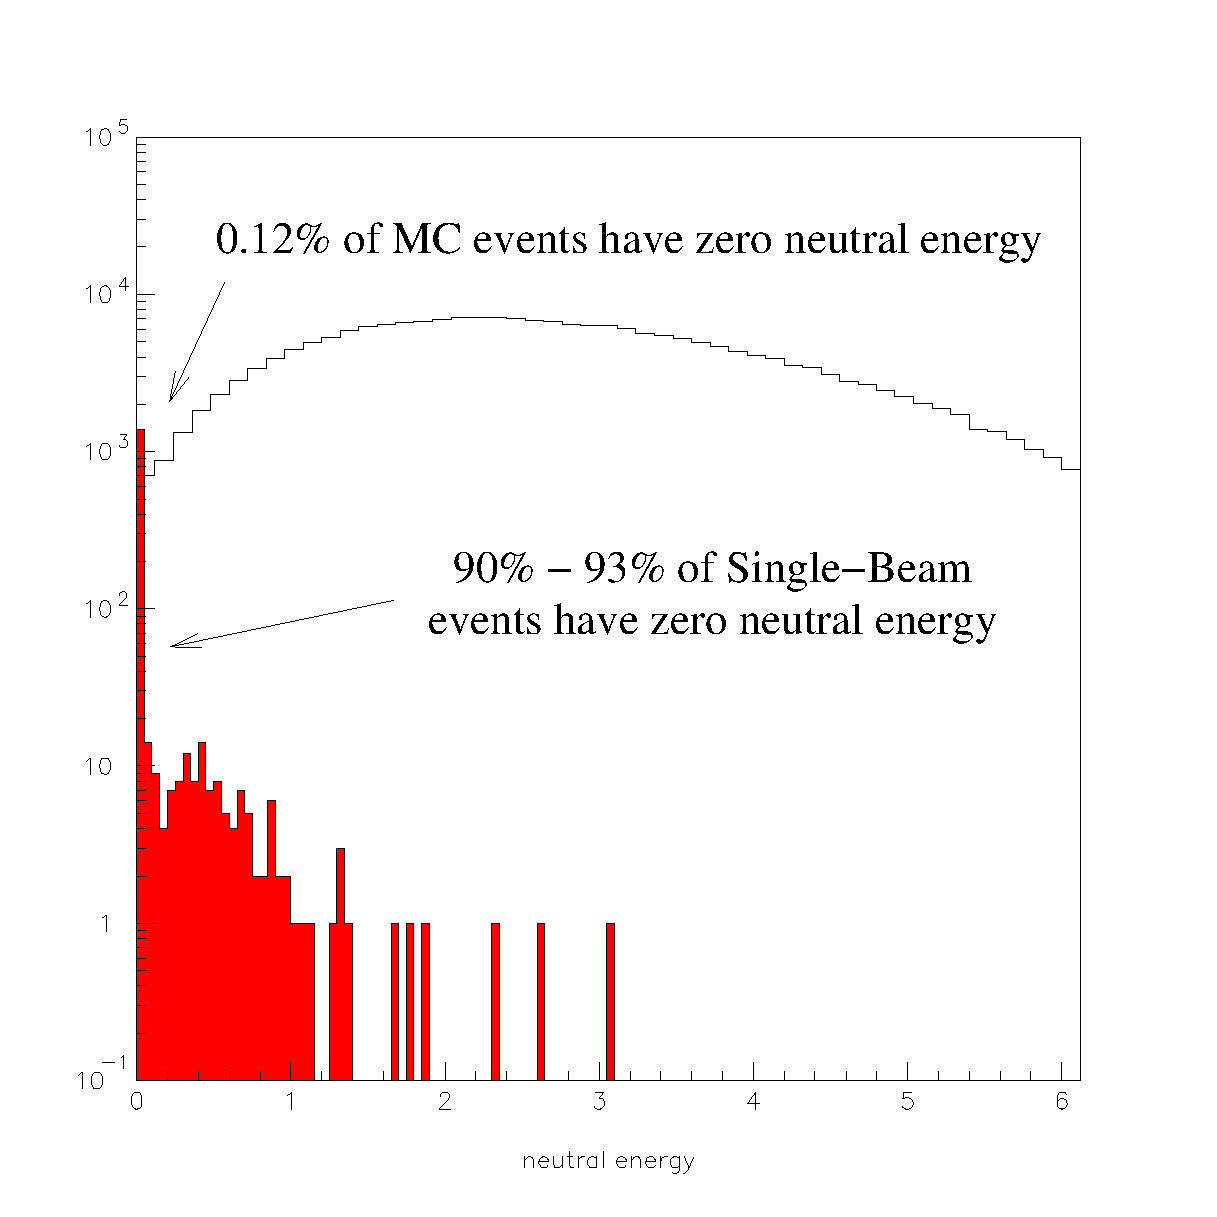
\includegraphics[width=\linewidth]{neutral_energy2.eps}
  \end{minipage}
\end{tabular}

\end{itemize}
\end{flushleft}

\vspace{0.5 cm}

\Large These cuts are now available in {\bf BeamGasFilterProc}.

\end{minipage}

\end{slide*}

%%%%%%%%%%%%%%%%%%%%%%%%%%%%%%%%%%%%%%%%%%%%%%%%%%%%%%%%%%%%%%%%%%%%%%%%%%%

%%%%%%%%%%%%%%%%%%%%%%%%%%%%%%%%%%%%%%%%%%%%%%%%%%%%%%%%%%%%%%%%%%%%%%%%%%%

\begin{slide*}

\slideframe{}
\slideframe*[\dkblue]{Oval}
\huge
\heading{Normalizing Contributions}

\begin{minipage}[t]{\linewidth}
\LARGE

\vspace{1 cm}

\begin{flushleft}
\begin{itemize}
  \item Continuum Hadrons: cross-section = 2.89 nb \\ \hspace{0.5 cm} (from R = 3.55)
  \item Tau Pairs: cross-section = 0.815 nb \\ \hspace{0.5 cm} (from first-order QED)
\end{itemize}
\end{flushleft}

\vspace{1 cm}

Problem: these need to be corrected for ISR, a factor of 6\% -- 22\%,
depending on acceptance of heavily-boosted events (assuming 3--4 GeV
cut-off).

\vspace{1 cm}

\begin{flushleft}
\begin{itemize}
  \item Two-Photon: Karl B.\ is developing a Monte Carlo to model
  these events. Preliminary cross-section = 0.18 nb.
  \item Beamgas? Measure in the data!
\end{itemize}
\end{flushleft}



\end{minipage}

\end{slide*}

%%%%%%%%%%%%%%%%%%%%%%%%%%%%%%%%%%%%%%%%%%%%%%%%%%%%%%%%%%%%%%%%%%%%%%%%%%%

\begin{slide*}

\slideframe{}
\slideframe*[\dkblue]{Oval}
\huge
\heading{Beamgas Normalization}

\begin{minipage}[t]{\linewidth}
\LARGE

There are two sources of charge asymmetry:

\begin{flushleft}
\begin{itemize}
  \item Track-counting issue in good, hadronic events
  \item Beamgas
\end{itemize}
\end{flushleft}

\begin{flushleft}
\begin{enumerate}
  \item \begin{tabular}{l c r}
  \begin{minipage}{3 in}
    Find pos/neg scale factor in the absence of beamgas.
  \end{minipage}
  & \hspace{0.5 in} & 
  \begin{minipage}{1.5 in}
    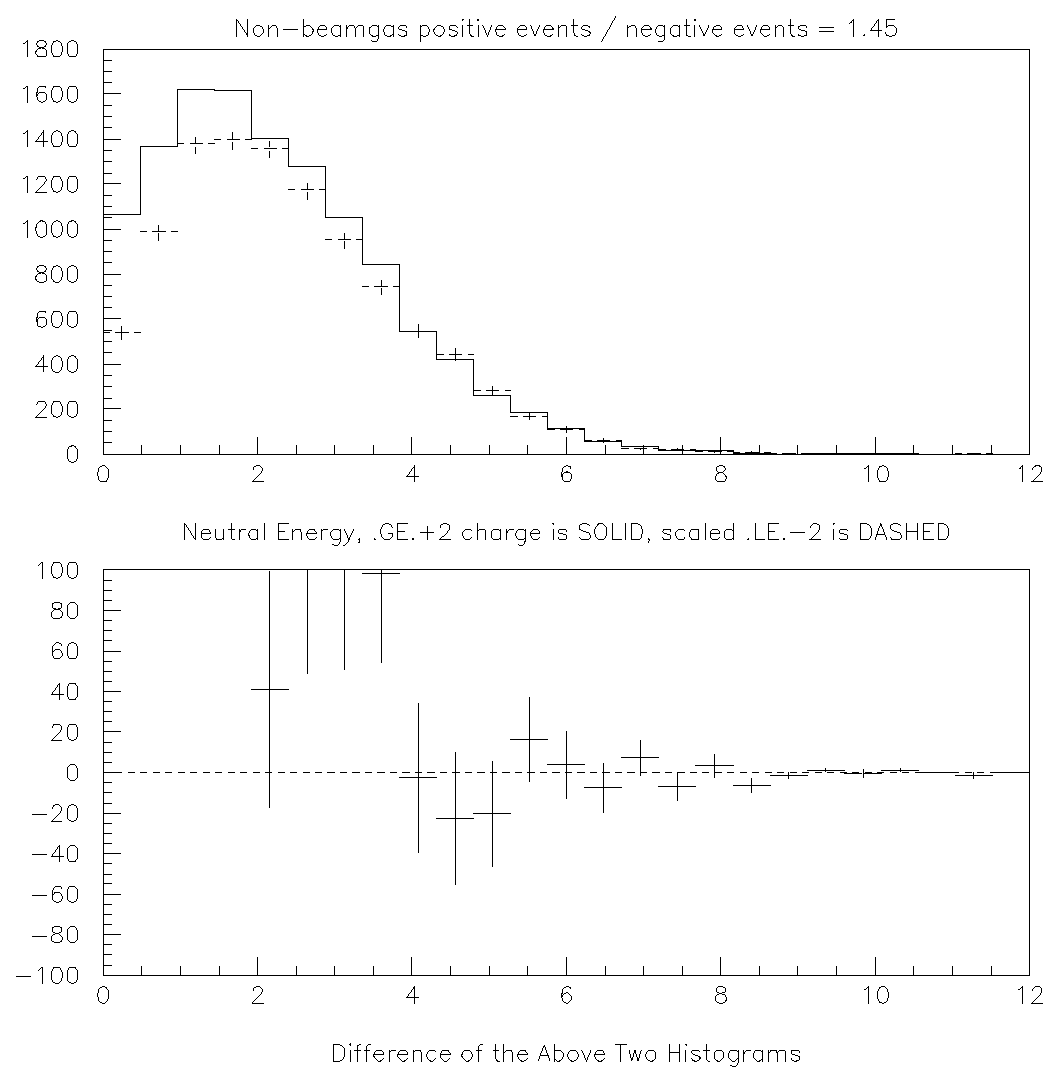
\includegraphics[width=\linewidth]{scale_non_beamgas.eps}
  \end{minipage}
\end{tabular}

  \item Do a weighted subtraction of $p_z$ distribution. Electrons
are forward-going and positrons backward-going: integrate for scale
factors. \\
  \begin{center}
    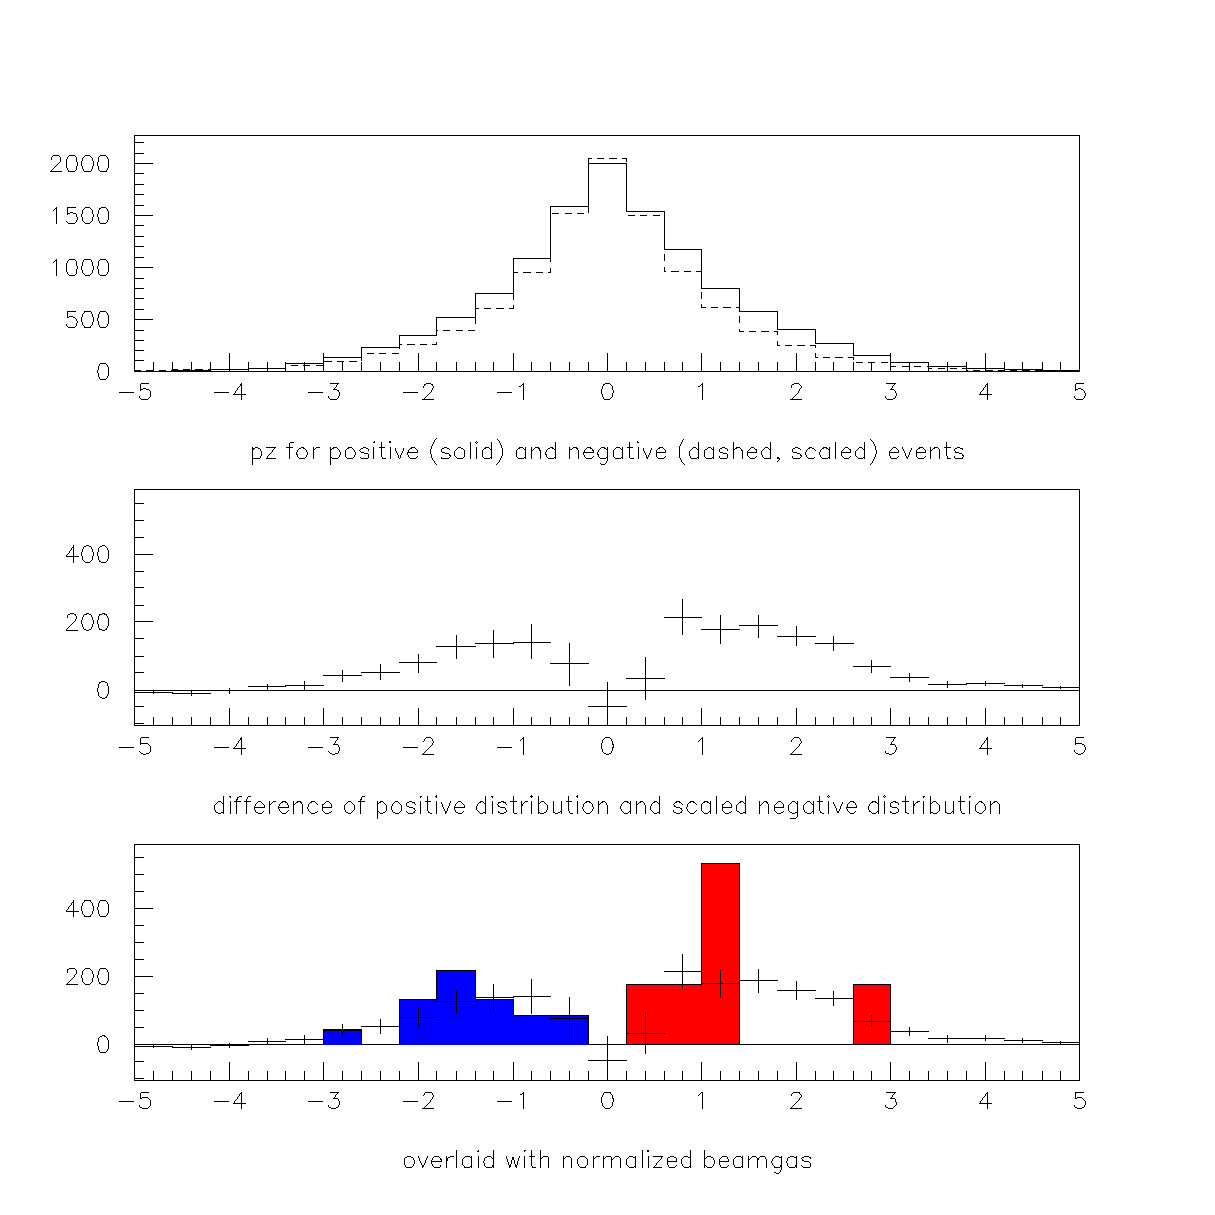
\includegraphics[width=0.5\linewidth]{beamgas_normalization.eps}
  \end{center}

\end{enumerate}
\end{flushleft}

\end{minipage}

\end{slide*}

%%%%%%%%%%%%%%%%%%%%%%%%%%%%%%%%%%%%%%%%%%%%%%%%%%%%%%%%%%%%%%%%%%%%%%%%%%%

%%%%%%%%%%%%%%%%%%%%%%%%%%%%%%%%%%%%%%%%%%%%%%%%%%%%%%%%%%%%%%%%%%%%%%%%%%%

\begin{slide*}

\slideframe{}
\slideframe*[\dkblue]{Oval}
\huge
\heading{Beamgas Normalization}

\begin{minipage}[t]{\linewidth}
\LARGE

Using these scale factors, we see that a wide variety of distributions
are in agreement.

\begin{center}
  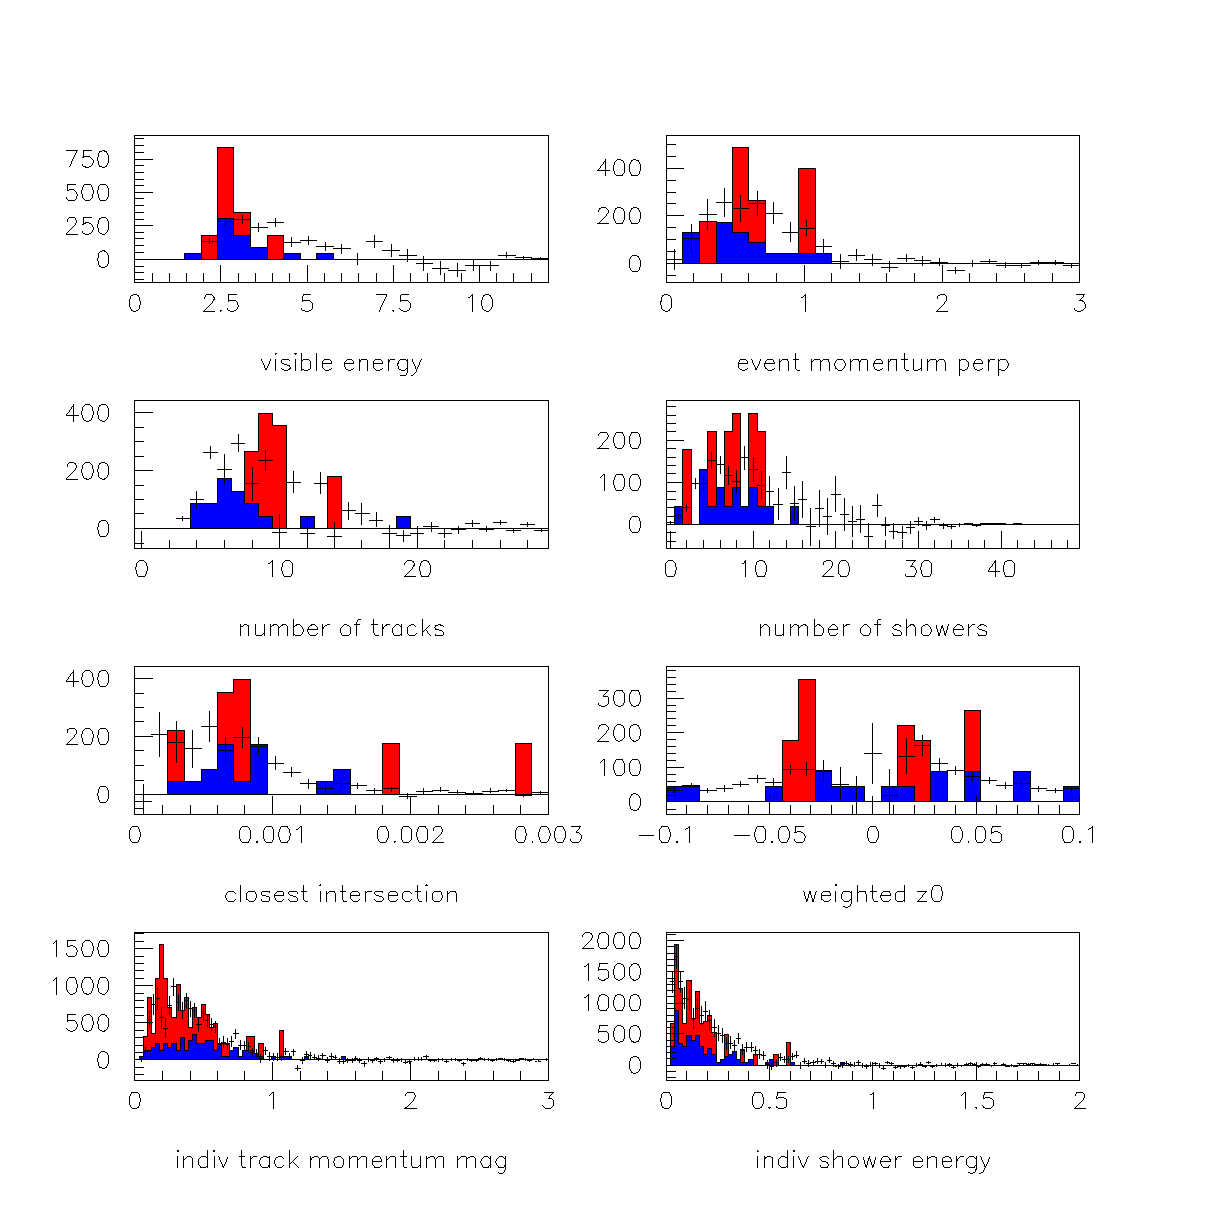
\includegraphics[width=0.80\linewidth]{beamgas_norm_is_good.eps}
\begin{minipage}{5 in}
$\longrightarrow$ evidence that there isn't a third source \\ \hspace{1 in} of charge
asymmetry!
\end{minipage}
\end{center}


\end{minipage}

\end{slide*}

%%%%%%%%%%%%%%%%%%%%%%%%%%%%%%%%%%%%%%%%%%%%%%%%%%%%%%%%%%%%%%%%%%%%%%%%%%%


%%%%%%%%%%%%%%%%%%%%%%%%%%%%%%%%%%%%%%%%%%%%%%%%%%%%%%%%%%%%%%%%%%%%%%%%%%%

\begin{slide*}

\slideframe{}
\slideframe*[\dkblue]{Oval}
\huge
\heading{Beamgas Normalization}

\begin{minipage}[t]{\linewidth}
\huge

Is the beamgas normalization, obtained from data, reasonable?

\vspace{0.5 cm}

\begin{center}
  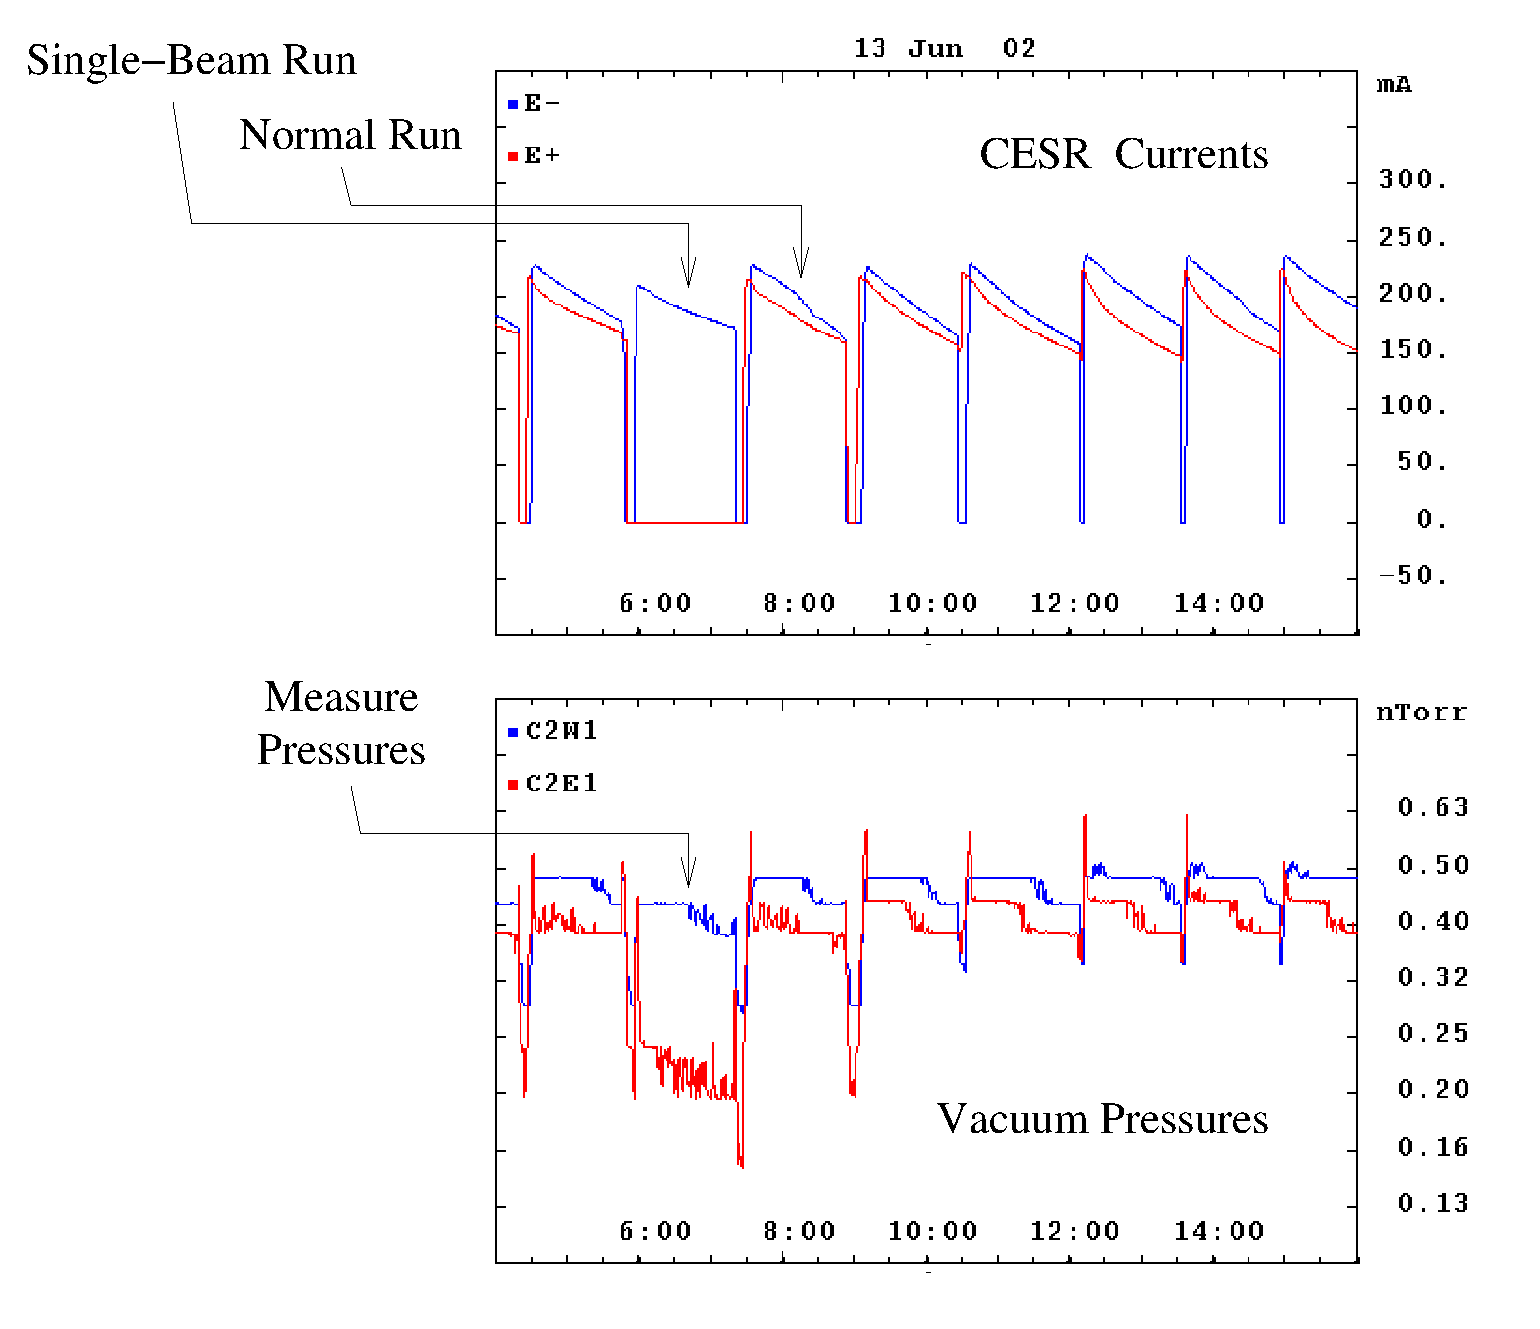
\includegraphics[width=0.7\linewidth]{beamgas_norm_is_reasonable.eps}
\end{center}

Scale by pressure $\times$ current
\begin{flushright}
$\Rightarrow$ electrons: 19.7, positrons: 64.3.
\end{flushright}

Scale by data $\Rightarrow$ electrons: 43.4, positrons: 177.

\end{minipage}

\end{slide*}


%%%%%%%%%%%%%%%%%%%%%%%%%%%%%%%%%%%%%%%%%%%%%%%%%%%%%%%%%%%%%%%%%%%%%%%%%%%

\begin{slide*}

\slideframe{}
\slideframe*[\dkblue]{Oval}
\huge
\heading{Charge Imbalance}

\begin{minipage}[t]{\linewidth}
\LARGE

\vspace{1 cm}

Okay, after correcting for instrumental net charge imbalance, what
remains is beamgas.  Why do I see an instrumental charge imbalance?

$\longrightarrow$ I have applied NO track quality cuts.

\vspace{1 cm}

What are the bad tracks? I.e.\ what is the cause and what track
quality cuts will restore symmetry in net charge?

$\longrightarrow$ I think they are multiple curlers and/or splashback
from the RICH.

$\longrightarrow$ $\big|$ d0 $\big|$ has a lot to do with it.

\vspace{1 cm}

Is this modelled correctly by the Monte Carlo?

$\longrightarrow$ No. Not without track quality cuts.

\end{minipage}

\end{slide*}

%%%%%%%%%%%%%%%%%%%%%%%%%%%%%%%%%%%%%%%%%%%%%%%%%%%%%%%%%%%%%%%%%%%%%%%%%%%

%%%%%%%%%%%%%%%%%%%%%%%%%%%%%%%%%%%%%%%%%%%%%%%%%%%%%%%%%%%%%%%%%%%%%%%%%%%

\begin{slide*}

\slideframe{}
\slideframe*[\dkblue]{Oval}
\huge
\heading{Conclusions}

\begin{minipage}[t]{\linewidth}
\LARGE

Estimating backgrounds with the new normalizations: \\
\begin{center}
  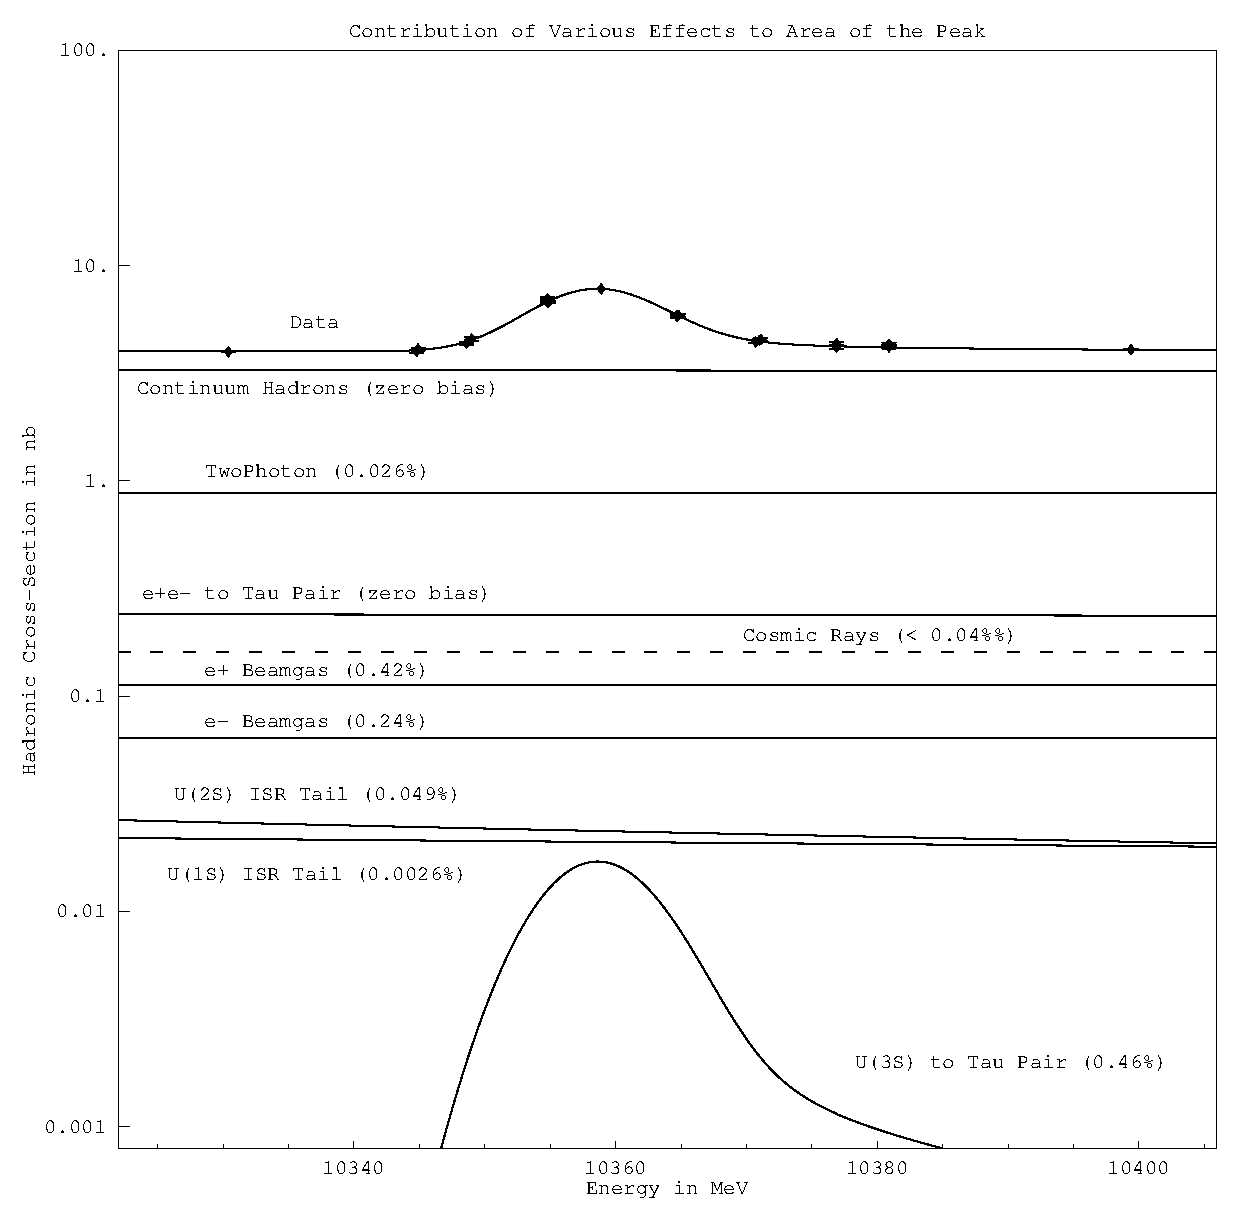
\includegraphics[width=0.8\linewidth]{all_backgrounds.eps}
\end{center}

Statistical uncertainty in area is 0.5\%.

Luminosity bias is 1.1\%.

\end{minipage}

\end{slide*}



\end{document}
